\documentclass[a4paper,12pt]{article}

% --- Packages ---
\usepackage{graphicx}
\usepackage{tikz}
\usepackage{geometry}
\usepackage{setspace}
\usepackage{titlesec}
\usepackage{everypage}



% --- Page setup ---
\geometry{top=1in, bottom=1in, left=1in, right=1in}
\setstretch{1.3}

\begin{document}

% ================= COVER PAGE =================
\thispagestyle{empty}

% --- Border Frame ---
\AddEverypageHook{%
\begin{tikzpicture}[remember picture,overlay]
  \draw[line width=1pt]
    ([xshift=1cm,yshift=-1cm]current page.north west)
    rectangle
    ([xshift=-1cm,yshift=1cm]current page.south east);
  \draw[line width=0.5pt,dashed]
    ([xshift=1.2cm,yshift=-1.2cm]current page.north west)
    rectangle
    ([xshift=-1.2cm,yshift=1.2cm]current page.south east);
\end{tikzpicture}}

% --- University Logo & Name ---
\begin{center}
    
\includegraphics[width=5cm]{image.png}\\[0.5cm]
\end{center}
\begin{center}
    {\LARGE \textbf{University of AJ\&K, Neelum Campus}} \\[0.3cm]
    {\Large Department of Computer Science \& IT} \\[0.8cm]
    \rule{0.75\textwidth}{1pt} \\[0.5cm]

    % --- Main Title (Subject + Assignment No) ---
    {\Large \bfseries Computer Networks} \\[0.3cm]
    { \bfseries Assignment No 2} \\[0.5cm]

    \rule{0.75\textwidth}{1pt} \\[1cm]
\end{center}

% --- Assignment Details ---
\vspace{3cm}
\begin{center}
    \begin{minipage}{0.45\textwidth}
        \centering
        \textbf{Submitted By:} \\[0.3cm]
        Jawad Ahmed
    \end{minipage}
    \hfill
    \begin{minipage}{0.45\textwidth}
        \centering
        \textbf{Submitted To:} \\[0.3cm]
        Sir Almas Sheikh
    \end{minipage}
\end{center}

% --- Footer with Date ---
\vfill
\begin{center}
    \rule{0.75\textwidth}{1pt} \\[0.3cm]
    {\large Submission Date: 4-Sept-2025} \\
\end{center}
\newpage
\begin{center}
    \rule{0.75\textwidth}{1pt} \\[0.5cm]
    {\Huge \bfseries Networking Commands} \\[0.3cm]
    \rule{0.75\textwidth}{1pt} \\[1cm]
\end{center}

\begin{enumerate}
    \item \textbf{ipconfig}
    \begin{itemize}
        \item \textbf{Purpose:} To display the basic IP configuration for all network adapters on a Windows machine.
        \item \textbf{Observation:} Shows my IP address, subnet mask, and default gateway for each adapter.
    \end{itemize}

    \item \textbf{ipconfig /all}
    \begin{itemize}
        \item \textbf{Purpose:} To display the full, detailed TCP/IP configuration for all adapters.
        \item \textbf{Observation:} Shows all basic info plus my MAC address, DHCP server, DNS servers, and lease information.
    \end{itemize}

    \item \textbf{ping $<IP>$}
    \begin{itemize}
        \item \textbf{Purpose:} To test connectivity to another network device and measure response time.
        \item \textbf{Observation:} Sends packets from my machine to the target IP and displays whether replies are received and how long they take.
    \end{itemize}
\begin{center}
    \fbox{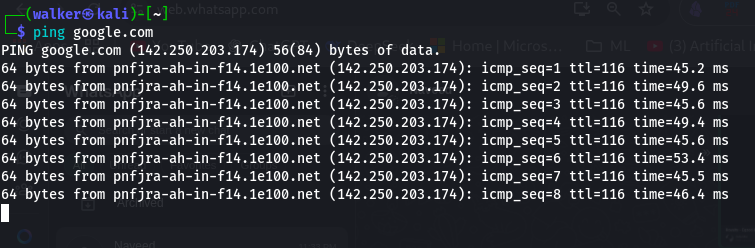
\includegraphics[width=15cm]{ping.png}}
\end{center}
    \item \textbf{arp -a}
    \begin{itemize}
        \item \textbf{Purpose:} To display the ARP table, which maps IP addresses to MAC addresses on the local network.
        \item \textbf{Observation:} Lists the IP and MAC addresses of devices my computer has recently communicated with.
    \end{itemize}

    \item \textbf{tracert $<hostname>$}
    \begin{itemize}
        \item \textbf{Purpose:} To trace the path packets take from my computer to a destination host.
        \item \textbf{Observation:} Lists all routers (hops) between my computer and the destination, showing the latency at each step.
    \end{itemize}

    \item \textbf{nslookup}
    \begin{itemize}
        \item \textbf{Purpose:} To query DNS servers to find the IP address of a domain name or the domain name of an IP address.
        \item \textbf{Observation:} Shows the DNS server my computer is using and the results of the query.
    \end{itemize}

    \item \textbf{netstat -a}
    \begin{itemize}
        \item \textbf{Purpose:} To display all active network connections and listening ports on the computer.
        \item \textbf{Observation:} Shows a list of all TCP and UDP connections to and from my computer and their current state.
    \end{itemize}

    \item \textbf{netstat -r}
    \begin{itemize}
        \item \textbf{Purpose:} To display the kernel's IP routing table.
        \item \textbf{Observation:} Shows the routing table on my computer, including network destinations, gateways, and interfaces.
    \end{itemize}

    \item \textbf{net view}
    \begin{itemize}
        \item \textbf{Purpose:} To display a list of computers and shared resources available on the network.
        \item \textbf{Observation:} Lists the names of other computers and servers visible on my local network.
    \end{itemize}

    \item \textbf{nbtstat -n}
    \begin{itemize}
        \item \textbf{Purpose:} To display NetBIOS names registered by the local computer.
        \item \textbf{Observation:} Shows the NetBIOS name table for my computer, including the registered names and services.
    \end{itemize}
\end{enumerate}

\newpage
\begin{center}
    \rule{0.75\textwidth}{1pt} \\[0.5cm]
    {\Huge \bfseries Networking Devices} \\[0.3cm]
    \rule{0.75\textwidth}{1pt} \\[1cm]
\end{center}

\centering
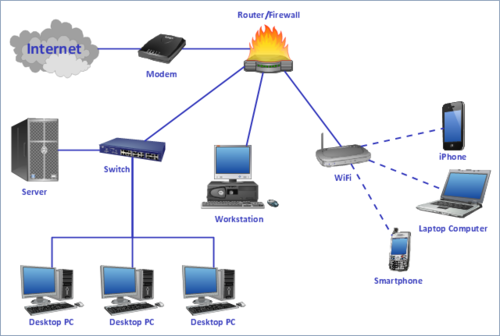
\includegraphics{cn.png}
\begin{enumerate}
    \item Find out the end devices and intermediary devices depicted in the scenario and place them rightly.\\

    \begin{center}
    \begin{tabular}{|l|l|}
        \hline
        \textbf{End Devices} & \textbf{Intermediary Devices} \\
        \hline
        PC & Switch \\
        Laptop & Router \\
        Server & Wireless Router / Access Point \\
        Printer & Cloud (representing WAN) \\
        IP Phone & \\
        \hline
    \end{tabular}
    \end{center}

    \item What is the difference between a hub, switch and a router? (Be specific).\\
    \begin{center}
    \begin{tabular}{|l|p{0.7\textwidth}|}
        \hline
        \textbf{Device} & \textbf{Function \& Difference} \\
        \hline
        \textbf{Hub} & Operates at Layer 1 (Physical). Broadcasts all data to every port, creating congestion. \\
        \hline
        \textbf{Switch} & Operates at Layer 2 (Data Link). Learns MAC addresses and sends data only to the specific destination port, reducing traffic. \\
        \hline
        \textbf{Router} & Operates at Layer 3 (Network). Connects different networks together and uses IP addresses to route packets between them. \\
        \hline
    \end{tabular}
    \end{center}

    \item Which networking devices are used in layer 1, 2 and 3 of TCP/IP model?\\
    \begin{center}
    \begin{tabular}{|l|l|l|}
        \hline
        \textbf{Layer \#} & \textbf{Layer Name} & \textbf{Devices used} \\
        \hline
        \textbf{1} & Network Interface & Hub, Repeater, Cables, Modem \\
        \hline
        \textbf{2} & Internet & Switch, Bridge, Network Card (NIC) \\
        \hline
        \textbf{3} & Transport/Application & Router, Multilayer Switch \\
        \hline
    \end{tabular}
    \end{center}

    \item My company wants to purchase some network hardware to which they can plug the 30 PCs in my department. Which type of network device is appropriate?\\
    a) A router\\
    b) A firewall\\
    c) A switch\\
    d) A server\\

    \textbf{Correct Option:} c) A switch\\
    \textbf{Explanation:} A switch is designed to connect multiple devices within a single Local Area Network (LAN) and efficiently manage traffic between them.\\

    \item I received a video file from my friend's Apple iPhone using AirDrop. What was his iPhone functioning as in that transaction?\\
    a) A server\\
    b) A client\\
    c) A Local Area Network\\

    \textbf{Correct Option:} a) A server\\
    \textbf{Explanation:} The iPhone was hosting and sending (serving) the file to my device, making it the server in this client-server transaction.\\

    \item What is my computer or smart phone functioning as when I watch a video from YouTube?\\
    a) A server\\
    b) An end-host\\
    c) A client\\

    \textbf{Correct Option:} c) A client\\
    \textbf{Explanation:} My device is requesting and receiving data from YouTube's servers, which makes it a client.\\

    \item My company wants to purchase some network hardware to connect its separate networks together. What kind of network device is appropriate?\\
    a) A firewall\\
    b) A host\\
    c) A LAN\\
    d) A router\\

    \textbf{Correct Option:} d) A router\\
    \textbf{Explanation:} A router's primary function is to connect different networks and route traffic between them.\\
\end{enumerate}


\end{document}